\chapter{System test}
This chapter presents the tests made throughout the project. 

\section{Unit tests}
Each module was developed separately and then tested before being added to the system. This made the process of combining all the blocks relatively smooth.\\
In this process we used uart a lot to debug. It is easy to use and provides a lot of insight when debugging. You can write specific messages on where in your code you are, or what values are in which registers etc.\\
When combining the blocks it is important to make sure everything is set up to use the same clock speeds and no pins overlap etc.

\section{Complete system test}
The Demoboard, we developed, was a central part of the complete system test. The complete system test comprised of taking the demoboard outside, wait until it had good satellite connection and then note the GPS coordinates. We also compared the heading on the display compass with a compass on the mobile phone. Below is a picture of the test setup:
\begin{figure}[H]
\centering
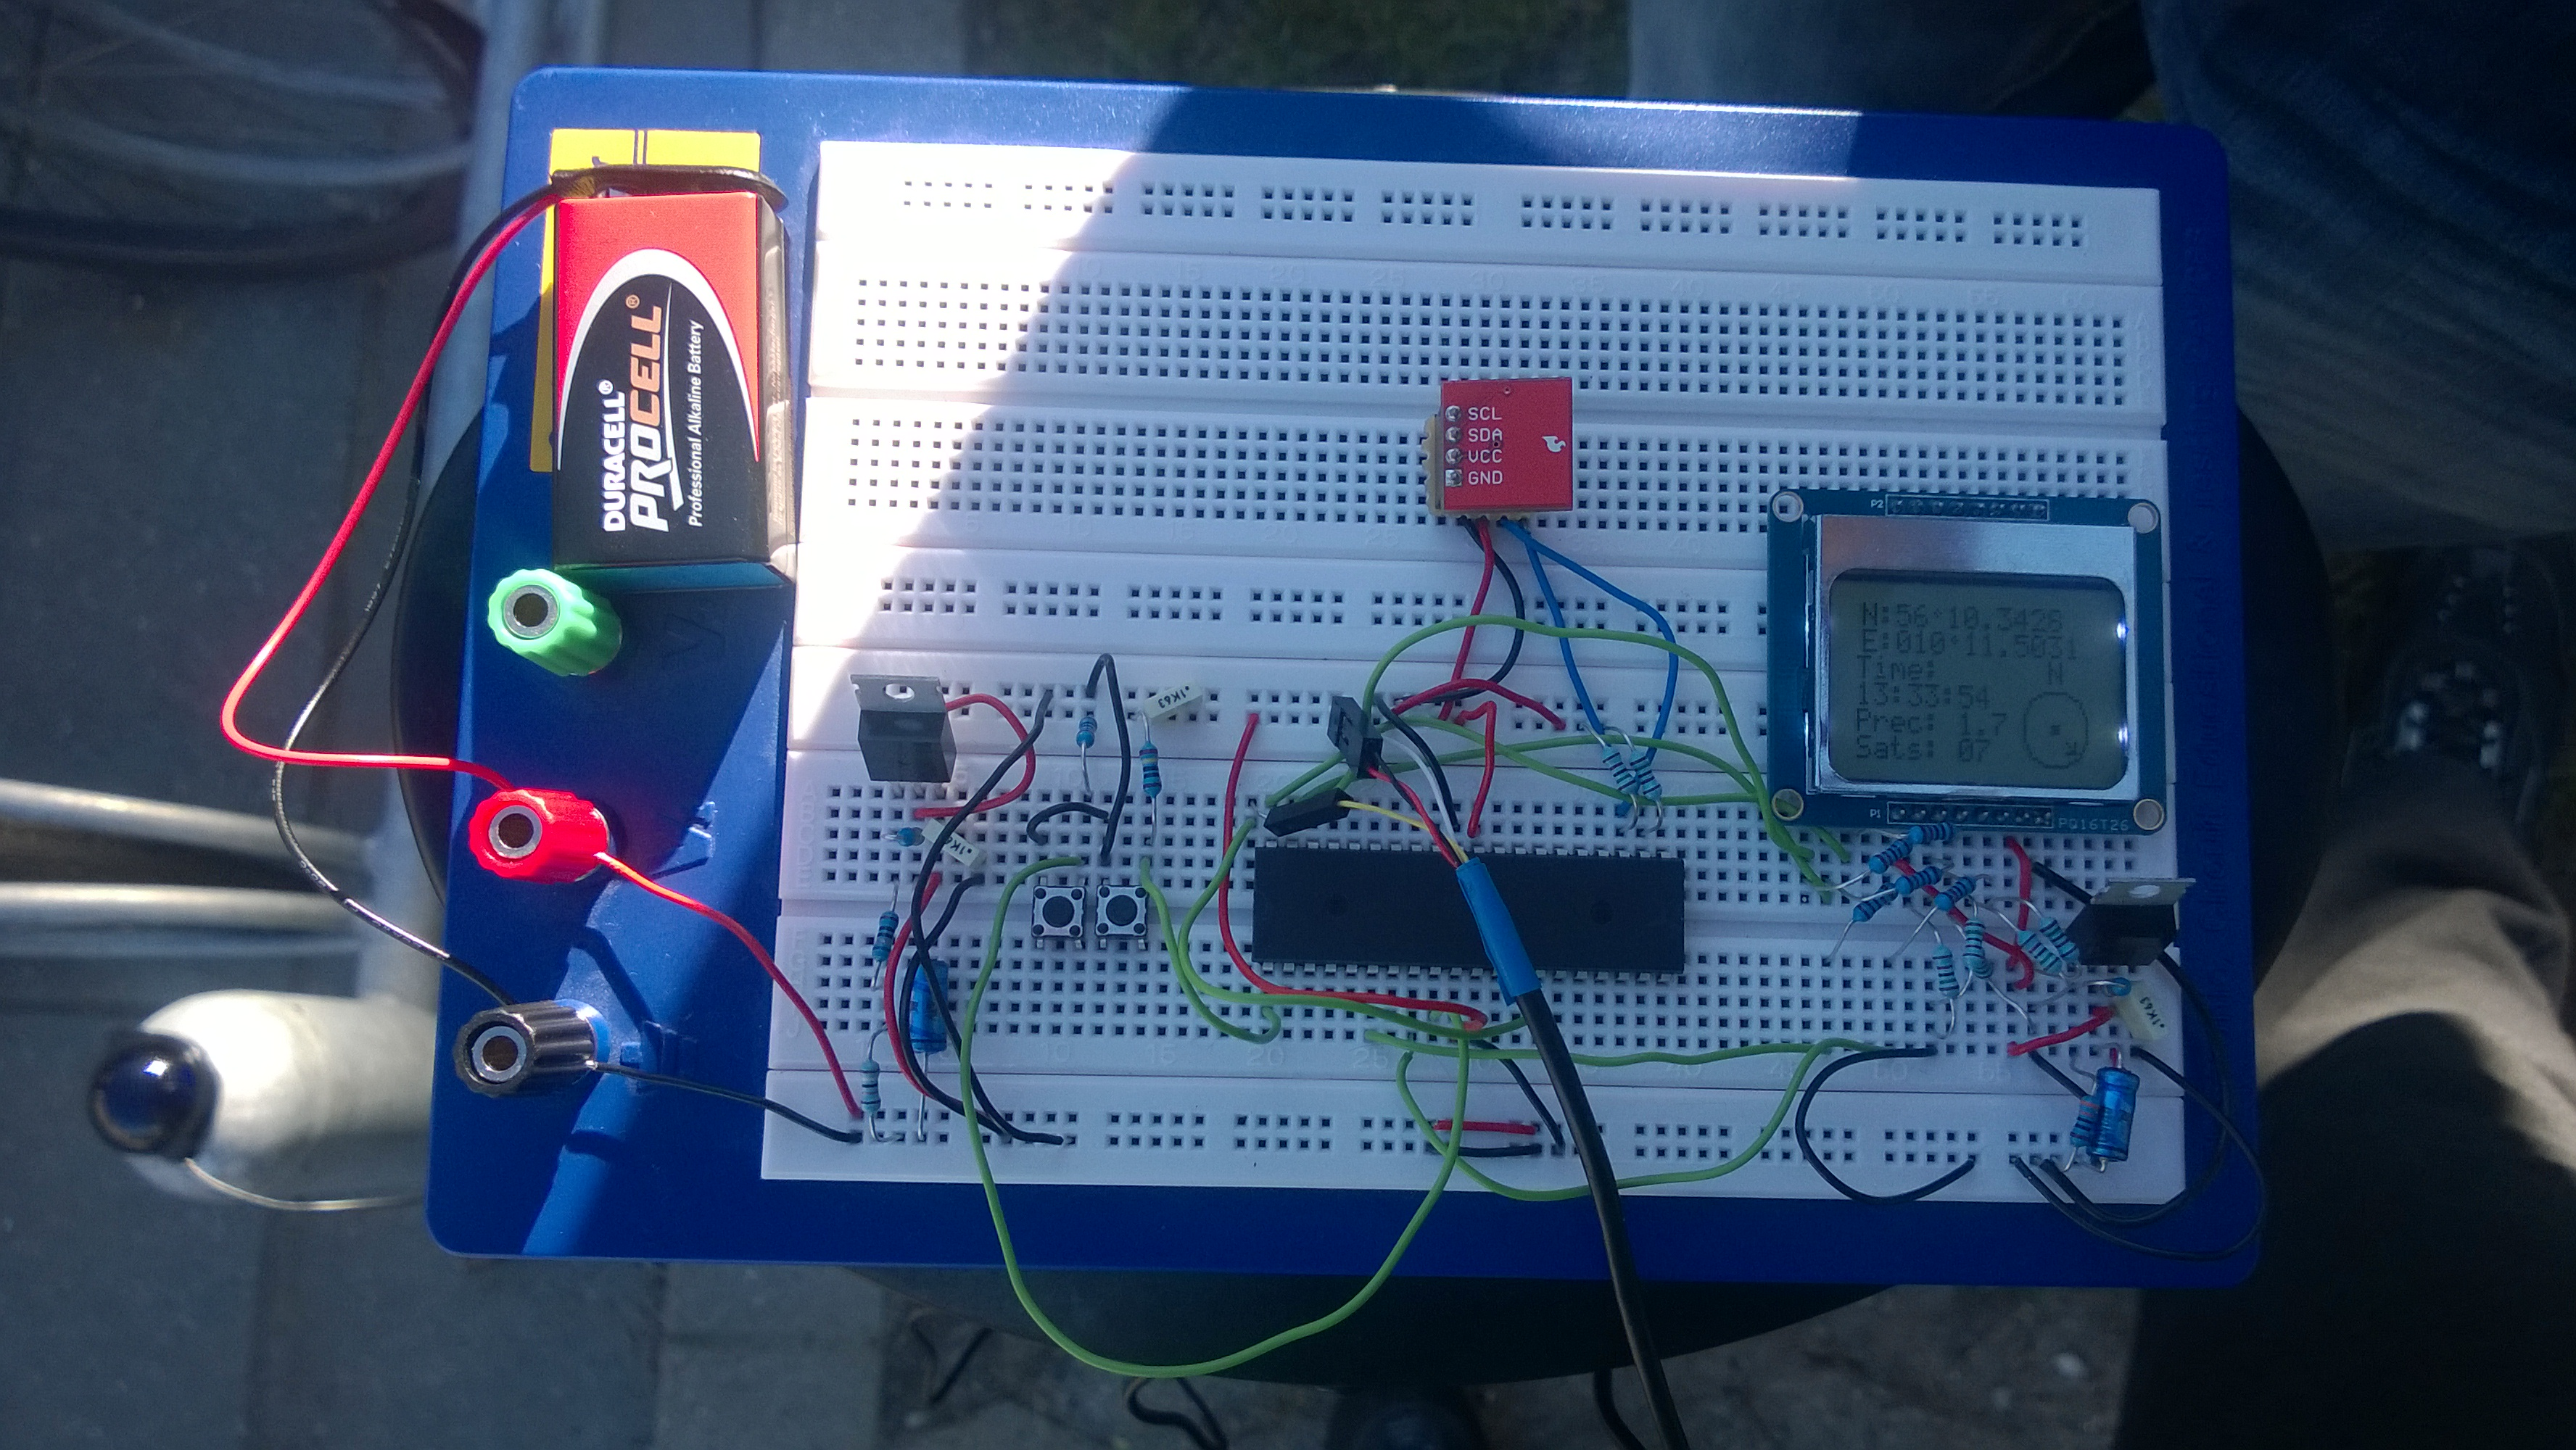
\includegraphics[width=.9\textwidth]{billeder/test_setup}
\caption{Picture of the test setup}
\end{figure}
On the picture the demobard is shown, and there is a clear read of the coordinates provided by the GPS module, which is seen as the black thing on the bicycle parking rack in the background.\\
The coordinates are:\\
$N:56^{\circ}10.3428$\\
$E:010^{\circ}11.5031$\\
Entering these coordinates in google maps we can get the location captured by the GPS module.

\begin{figure}[H]
\centering
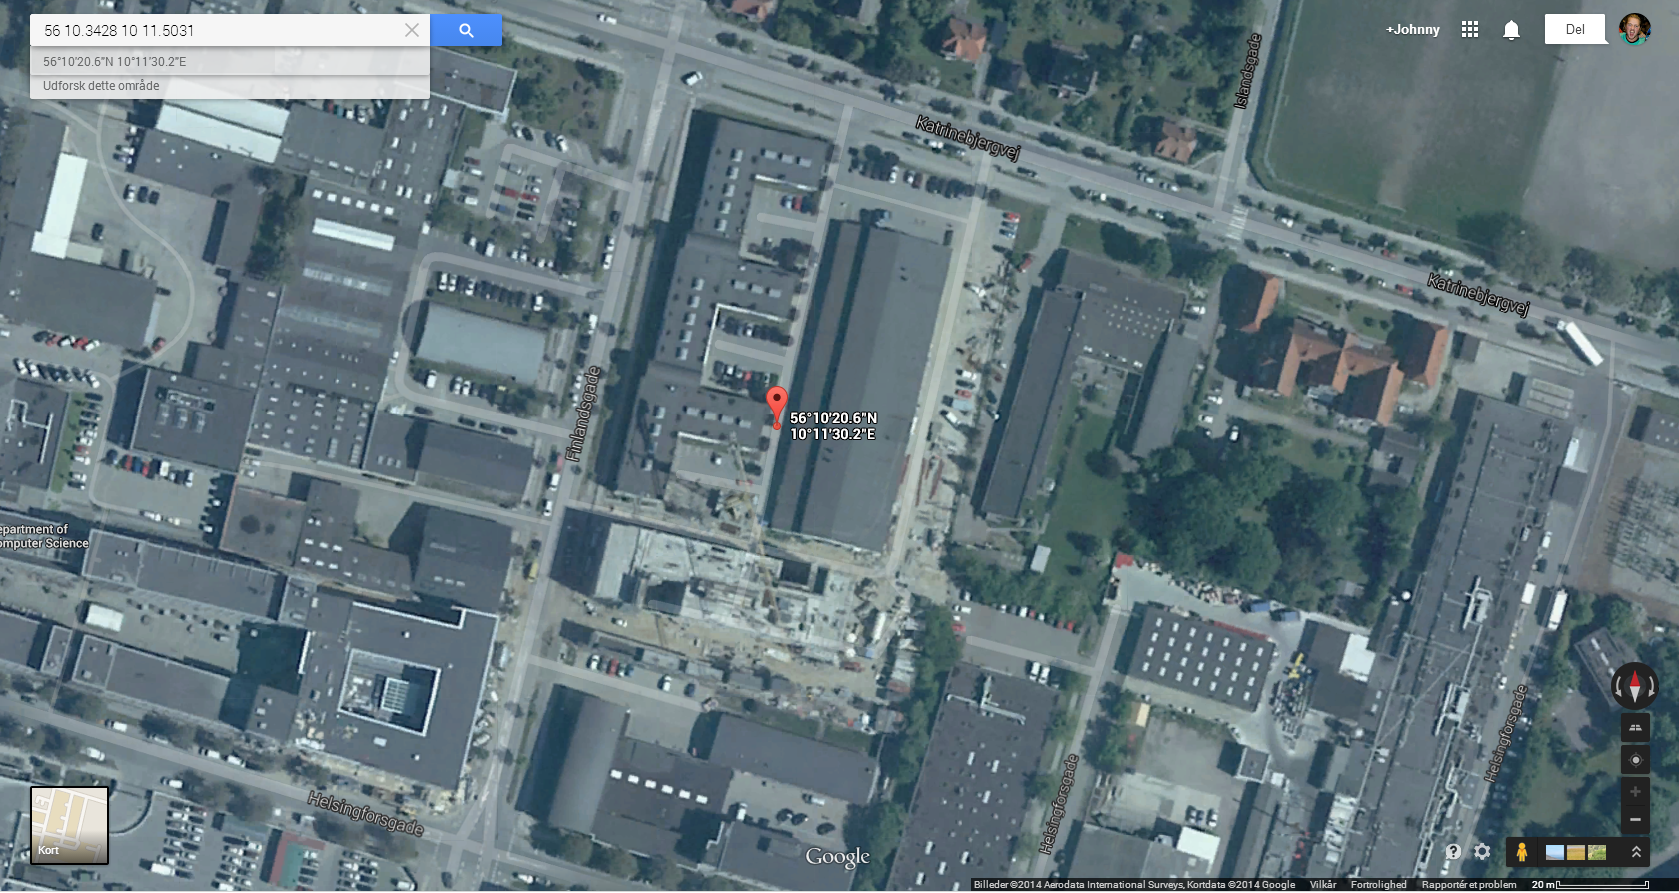
\includegraphics[width=.9\textwidth]{billeder/coordinate_map}
\caption{Test setup result plotted with google maps}
\end{figure}

In this test we had a precision of approximately $\leq1$ meter.
Below is shown a test picture of the compass heading.
\begin{figure}[H]
\centering
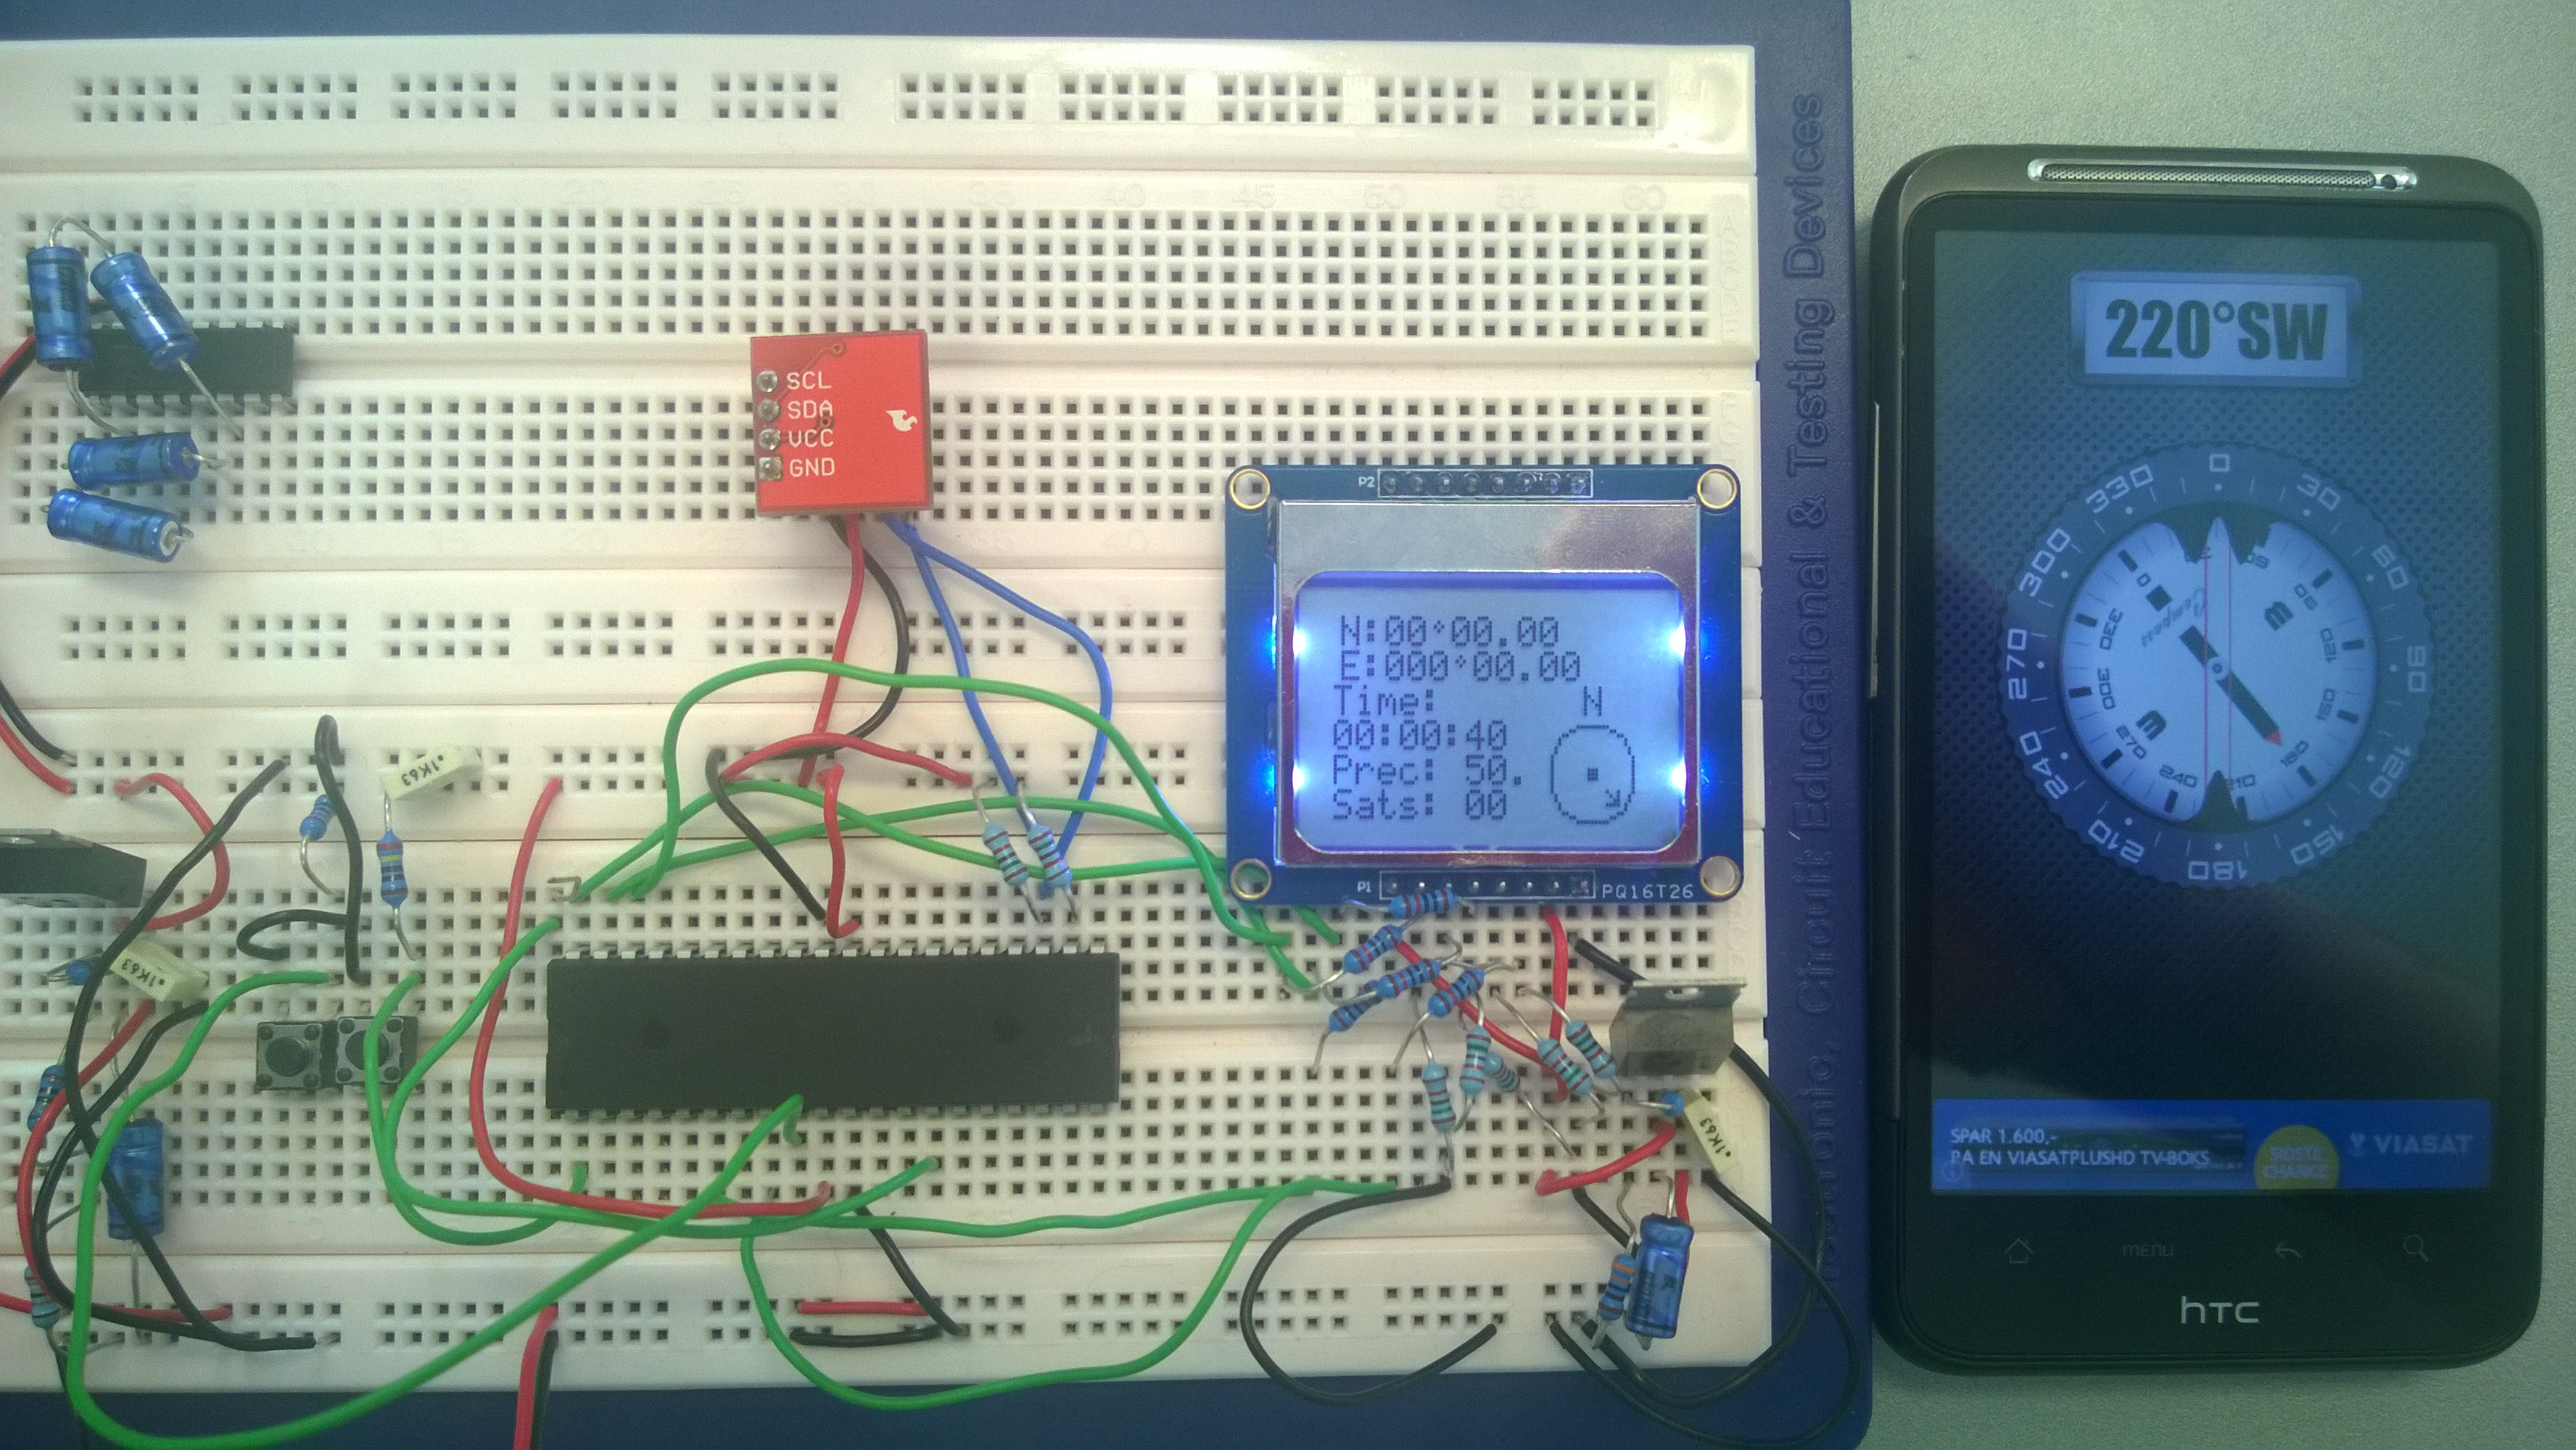
\includegraphics[width=.9\textwidth]{billeder/compas}
\caption{Comparison of mobile compass heading and GeoDude compass heading}
\end{figure}
\section{Improvements}
%Få RTOS optimeret
If we were to add hardware modules or features to our project we would have to look at the delay times in our RTOS tasks. Substantial work would go into optimising every task delay time to achieve the smoothest, most optimised system. This is something that can be done in the future. Adding RTOS elements like "suspend" and "resume" can further improve the system as there is no need to update the display if there is no new data as an example. \\
Another improvement we though of, but didn't implement, was to power down all peripherals before entering the boot loader and light an LED. This would be a good practice because it is not being used, and the GPS module would interfere on the UART connection used for the boot loader.

\chapter{Obtained experience}
\textbf{Screen:}\\
Working with the nokia 3310 screen we have learned to properly read a datasheet, timing diagrams etc. The screen interface is similar although not perfectly the same to screens we have been working with in class.\\
We also learned to make custom graphics to the screen used to display the compass arrow.

\textbf{Magnetometer:}\\
The magnetometer was quite simple to work with, since it had few settings and a simple output we know very well (degrees).

\textbf{GPS:}\\
By working with the GPS module we have acquired a working knowledge of the NMEA-0183 standard and how modules that utilise this standard interface and operate. 

\textbf{Boot Loader:}\\
When we first worked with boot loading it seemed simple enough, but after working with boot loading we have understood just how useful it is, as it saved us a lot of time and hassle. We also learned how the boot loader works with regards to the functionality of the code and the structure of the boot loader.

\textbf{FreeRTOS:}\\
We have already worked with FreeRTOS in the exercise but implementing it in our own system has given us an understanding of the advantages of using a real time operating system. FreeRTOS also uses up some space in memory so we learned how to allocate memory better for it run optimally.


%%%%%%%%%%%%%%%%
%% konklusion %%
%%%%%%%%%%%%%%%%
\chapter{Conclusion}
The project has given the group a working knowledge of several disciplines within microcontrollers and interfacing with various communication buses and modules.\\
The group have implemented the system with an ATmega32 on a breadboard, successfully interfacing a screen, a magnetometer and a GPS-module, all previously unknown to the group members. The ATmega32 runs FreeRTOS and has working boot loader functionality.\\
Although the time frame for the project has been very short the group feels a lot have been achieved during this time.\\
It is nice to see a project through once in a while.






%We conclude on a successful short time development project. Throughout the project we have developed in AVRStudio 6 and implemented on the ATmega32. 
%
%We implemented the system with an ATmega32 on a breadboard with a screen, a magnetometer and a GPS module. The ATmega32 has FreeRTOS running. Programming the ATmega32 is done with a boot loader after a button is pressed.
%
%We can conclude on a project with an working expandable basis system as result. The screen displays the data we chose in the project boundary and updates atleast every second. 
%
%We are happy to conclude this project with a working product.

